\section{Gestion des enseignements}

\begin{center}
\scalebox{0.7}{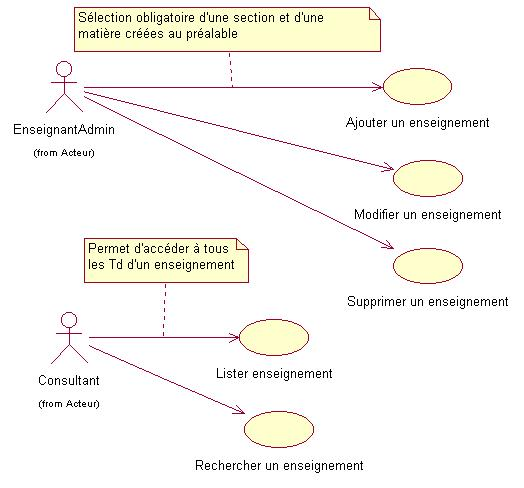
\includegraphics{images/enseignement.jpg}}\\
\par{Package Gestion Enseignement}
\end{center}
Voici les diff{\'e}rents sc{\'e}narios:\\

	\begin{itemize}
	\item Consultant
		\begin{itemize}
		\item Rechercher un enseignement :
			\begin{itemize}
			\item Pr{\'e}-requis : Il doit exister au moins un enseignement
			\item Description : Il selectionne l'option {\it Rechercher un enseignement}.\\
			il saisie au choix l'ann{\'e}e, la section, et la mati{\`e}re. 
			\item Post-requis : Affiche tous les tds et les projets en relation avec l'enseignement sous forme de liste.
			\end{itemize}


	\item Enseignant
		\begin{itemize}
		\item Creer un enseignement :
			\begin{itemize}
			\item Pr{\'e}-requis : Etre log{\'e}, avoir des mati{\`e}res et des sections d{\'e}j{\`a} existant. 
			\item Description : Il s'identifie avec son login et son mot de passe. \\
			Il saisie une ann{\'e}e et s{\'e}lectionne successivement une section et une mati{\`e}re.\\
			Il d{\'e}signe le nom du nouvel enseignement qu'il veut cr{\'e}er. Il valide ses choix.
			\item Post-requis : Un nouvel enseignement est cr{\'e}{\'e}.
			\end{itemize}
		\end{itemize}
	\end{itemize}


	\item Administrateur
		\begin{itemize}
		\item D{\'e}placer vers la corbeille un enseignement :
			\begin{itemize}
			\item Pr{\'e}-requis : Etre log{\'e}. Il doit exister au moins un TDs ou projets.\\
			\item Description : IL d{\'e}place les TDs ou les projets vers la corbeille.\\
			 C'est en fait une suppression partiel car ils peuvent {\^e}tre restaur{\'e} tant que l'administrateur ne l'a pas supprim{\'e} totalement\\
			\item Post-requis : Le Td ou le projet d{\'e}plac{\'e} n'est plus dans le liste des tds ou des projets.
			\end{itemize}
		\end{itemize}
	
		\begin{itemize}
		\item Suppression totale de l'enseignement:
			\begin{itemize}
			\item Pr{\'e}-requis : Etre log{\'e}. Il doit exister au moins un TDs ou projets dans la corbeille.\\
			\item Description : Il selectionne le projet ou le td qui veut supprimer et valide la suppresion.\\
			\item Post-requis : Le projet ou le td est compl{\`e}tement supprim{\'e}. Il est irr{\'e}cup{\'e}rable.
			\end{itemize}
		\end{itemize}
		\begin{itemize}	
		\item Restaurer l'enseignement:
			\begin{itemize}
			\item Pr{\'e}-requis : Etre log{\'e}. Il doit exister au moins un TDs ou projets dans la corbeille.\\
			\item Description : Il selectionne le projet ou le td qui veut restaurer et valide restauration.\\
			\item Post-requis : Le projet ou le td est restaur{\'e} a l'endroit ou il {\'e}tait avant suppression avec les options qu'il avait avant suppression
			\end{itemize}
		\end{itemize}


	\end{itemize}


\newpage
Voyons maintenant les priorit{\'e}s des diff{\'e}rentes actions quant au
d{\'e}veloppement du logiciel.\\\\\\
\begin{tabular}{|p{4cm}|c|p{4cm}|p{5cm}|}
\hline
  Fonction & Priorit{\'e} & Qualit{\'e} & Mesure \\
\hline
Ajouter un enseignement & 5 & Facile & Utilisation de menus simples.\\
\hline
Modifier un enseignement & 3 & Facile et Fiable & Utilisation de menus
  simples et coh{\'e}rence avec les devoirs. \\
\hline
Supprimer un enseignement & 4 & Fiable et S{\^u}r & Ne pas supprimer un autre
  ensignement que celui s{\'e}lectionn{\'e}. Les devoirs de l'enseignement
  sont archiv{\'e}s. \\
\hline
Lister les enseignements & 5 & Rapide et Fiable & Efficace. Affichage
  de tous les enseignements sans omissions ni redondances.\\
\hline
Rechercher un enseignement & 3 & Facile et Rapide & Recherche par mots
  cl{\'e}s et efficace.\\
\hline
\end{tabular}
\begin{center}
{\'e}chelle de mesure de la priorit{\'e}:

\scalebox{0.5}{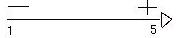
\includegraphics{images/echelle.jpg}}
\end{center}
